\documentclass[report]{res} 
\usepackage{hyperref}
\usepackage{array}
\usepackage{graphicx}
\usepackage{listings}
\hypersetup{
	colorlinks=true,
	linkcolor=blue,
	filecolor=magenta,      
	urlcolor=blue,
}

\urlstyle{same}



\begin{document}
	
	\begin{titlepage}
		
		\newcommand{\HRule}{\rule{\linewidth}{0.5mm}} % Defines a new command for the horizontal lines, change thickness here
		
		\center % Center everything on the page
		
		%----------------------------------------------------------------------------------------
		%	HEADING SECTIONS
		%----------------------------------------------------------------------------------------
		{\LARGE e-Yantra Summer Internship Programme 2015}\\[1.5cm] 
		{\Large IIT Bombay}\\[1cm] % Major heading 
		{\large Dcumentation}\\
		
		
		%----------------------------------------------------------------------------------------
		%	TITLE SECTION
		%----------------------------------------------------------------------------------------
		
		\HRule \\[0.4cm]
		{ \huge \bfseries PID based Path Planning }\\[0.4cm] % Title of your document
		\HRule \\[4cm]
		
		%----------------------------------------------------------------------------------------
		%	AUTHOR SECTION
		%----------------------------------------------------------------------------------------
		
		\begin{minipage}{0.4\textwidth}
			\begin{flushleft} \large
				\emph{Interns: }\\
			\end{flushleft}
			
			\begin{flushleft}
				{\large Dhirendra Sagar} \\  Email:sagar.dhirendra@gmail.com \\ Mob: 8858643336
			\end{flushleft}
			
			\begin{flushleft}
				{\large Uttam Kumar Gupta} \\  Email:23guptageek@gmail.com	\\Mob: 9473735800 \\
			\end{flushleft}
			
		\end{minipage}
		~
		\begin{minipage}{0.4\textwidth}
			
			\begin{flushright} \large
				\emph{Mentor:} \\
			\end{flushright}
			
			\begin{flushright}
				{\large Amiraj Dhawan\\} 
			\end{flushright}
		
		\end{minipage}\\[2cm]
		
		% If you don't want a supervisor, uncomment the two lines below and remove the section above
		%\Large \emph{Author:}\\
		{ Under the guidance of\\ \large{ Prof.Kavi Arya\\[3cm]}} % Your name
		
		%----------------------------------------------------------------------------------------
		%	DATE SECTION
		%----------------------------------------------------------------------------------------
		
		{\large 5 June 2015  \\ to \\ 8 July 2015}\\[3cm] % Date, change the \today to a set date if you want to be precise
		
		%----------------------------------------------------------------------------------------
		%	LOGO SECTION
		%----------------------------------------------------------------------------------------
		
		%\includegraphics{Logo}\\[1cm] % Include a department/university logo - this will require the graphicx package
		
		%----------------------------------------------------------------------------------------
		
		\vfill % Fill the rest of the page with whitespace
		
	\end{titlepage}

	\begin{quote}
		\centering \textbf{\Huge Contents}
	\end{quote}
	\qquad \\ \\
	
	\begin{enumerate}
	
		\item \textbf{\Large Abstract}
		\item \textbf{\Large Objective of the work}
		\item \textbf{\Large Completion}
		\item \textbf{\Large Tools required}
		\item \textbf{\Large Introduction}
		\item \textbf{\Large Theme description}
		\item \textbf{\Large Algorithmn}
		\item \textbf{\Large Implementation}
		\item \textbf{\Large Flow chart}
		\item \textbf{\Large Results and discussion}
		\item \textbf{\Large Problems Faced}
		\item \textbf{\Large References}
		
	\end{enumerate}
	
	\pagebreak
	
	
	\begin{center}
		\textbf{\huge Abstract} \\
	\end{center}
    
    \begin{itemize}
    	
    \item In this project we used PID controller to control the movements of Firebird V using image processing on frames of captured video. 
    \item We detected target and source position on the basis of their colors then source follows a path towards target point with controlled motion so that it did not deviate from its path.
    \item When firebird V is deviated from its path, PID controller controls the left and right motor speed, accordingly it tried to regain its path as fast as possible and gives smoother movements.
	
	\end{itemize}
	
	\pagebreak
	
	
	\begin{center}
		\textbf{\huge Objective of the work} \\
	\end{center}
	
	The aim of the project is to detect the Firebird V robot using image processing in an arena and given a moving end location, plan the robot's motion using PID closed loop feedback system. The arena will contain fixed obstacles. \\
	
	\begin{tabular}{|c|c|c|}
	
		\hline
		\bf Sr.No & \bf Tasks & \bf Deadline \\ 
		\hline
		1.) & Learning firebird V programming and PID controller & 2 days \\
		\hline
		2.) & Develop Motion commands (Xbee communication) & 1 days \\
		\hline
		3.) & Detection of Firebird V using image Processing and Map the Path for destination position & 5 days\\
		\hline
		4.) & Implement the PID controller and Tune it & 5 days
		\\ \hline
		5.) & Testing/Documentation(usage Manual, Documented Code) & 5 days
		\\ \hline
		
	\end{tabular} \\ \\
	
	\pagebreak


	\begin{center}
		\textbf{\huge Tools Required} \\
	\end{center}

	\begin{itemize}
		\item Installed the following libraries:

		\begin{itemize}

			\item \textbf{Atmel Studio 6.0}: For embedded C programming 
			\item \textbf{Python 2.7}: Python 2.7 IDLE is used for python programming. 
			\item \textbf{openCV}: This library provides various modules which are used for processing an image. color masking and contours detection etc, is done by it.
			\item \textbf{numpy}: numpy used to handle array in python.
			\item \textbf{X-CTU}: For configuration of xbee modules to send motion commands from laptop to firebird V.
			\item \textbf{pyserial}: To send command using xbee serial communication through python.
			
		\end{itemize}	
		
	\end{itemize}
	
	\pagebreak
	
	
	\begin{center}
		\textbf{\huge Introduction} \\
	\end{center}
	
	\textbf{HSV}:
	
	The first thing we usually notice about a color is its hue.   Hue describes the shade of color and that color is found in the color spectrum. Red, yellow, and purple are words that describe hue. The next most significant aspect of color is the saturation,S. The saturation describes how pure the hue is with respect to a white reference.The next thing is brightness or value.This is a relative description of how much light is coming from the color. If the color reflects a lot of light, we would say that it is bright.\\
	
	\begin{center}
	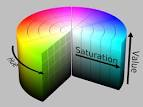
\includegraphics{graphics/hsv.jpg}
	\end{center}
	
	\textbf{Masking }:
	A mask is a black and white image of the same dimensions as the original image (or the region of interest you are working on). Each of the pixels in the mask can have therefore a value of 0 (black) or 1 (white). 
	When executing operations on the image the mask is used to restrict the result to the pixels that are 1 (selected, active, white) in the mask. In this way the operation restricts to some parts of the image.
	
	\textbf{Dilation (Morphology Operation) } :
	This operations consists of convoluting an image   with some kernel ( ), which can have any shape or size, usually a square or circle. The kernel   has a defined anchor point, usually being the center of the kernel. As the kernel is scanned over the image, we compute the maximal pixel value overlapped by and replace the image pixel in the anchor point position with that maximal value. As you can deduce, this maximizing operation causes bright regions within an image to “grow” (therefore the name dilation). Take as an example the image above. Applying dilation we can get:\\	
	
	\begin{center}
	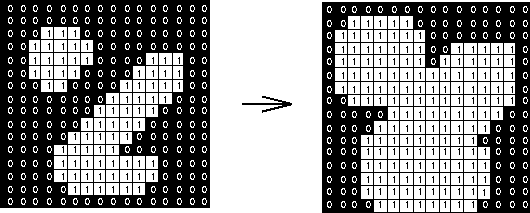
\includegraphics[scale = 1]{graphics/dilation.png}
	\end{center}
		
	The background (bright) dilates around the black regions of the letter.
	Closing
	•	It is obtained by the dilation of an image followed by an erosion.
	
	•	Useful to remove small holes (dark regions).
	
	
	\textbf{Contours}:
	
	The contours are a useful tool for shape analysis, object detection and recognition of detected contours. Each contour is stored as a vector of points.
	
	\begin{lstlisting}
	cv2.findContours(image, mode, method[, contours[, hierarchy[, offset]]]) → contours, hierarchy\\
	\end{lstlisting}
	
	\begin{lstlisting}
	cv2.drawContours(image, contours, contourIdx, color[, thickness[, lineType[, hierarchy[, maxLevel[, offset]]]]]) → None
	\end{lstlisting}
	
	\textbf{Heapq Algorithm}:
	
	A heap is a tree-like data structure where the child nodes have a sort-order relationship with the parents. Binary heaps can be represented using a list or array organized so that the children of element N are at positions 2*N+1 and 2*N+2 (for zero-based indexes). This layout makes it possible to rearrange heaps in place, so it is not necessary to reallocate as much memory when adding or removing items.
	A max-heap ensures that the parent is larger than or equal to both of its children. A min-heap requires that the parent be less than or equal to its children. Python’s heapq module implements a min-heap.\\
	
	\textbf{Accessing Contents of Heap}:
	
	Once the heap is organized correctly, use heappop() to remove the element with the lowest value. In this example, taken from the stdlib documentation, heapify() and heappop() are used to sort a list of numbers.
	
	\textbf{PID controller}:
	
	\begin{itemize}
	
	\item	PID is an acronym for Proportional Integral Derivative.
	\item	Main task of the PID controller is to minimize the error of whatever we are controlling.
	\item	PID takes input, calculates the deviation from the intended behaviour and accordingly adjusts the output so that deviation from the intended behaviour is minimized and greater accuracy obtained.
	\item	As the name suggests, PID algorithm consists of three basic coefficients: proportional, integral and derivative which are varied to get optimal response. 
	\\ \\The basic terminology we use to implement the PID Controller are:
	\item	Error(e): The error is the amount by which robot is deviating from it’s set-point.
	\item	Proportional(P): The proportional component depends only on the difference between the set point and the process variable. This difference is referred to as the Error term.
	\item	Integral(I): The integral component sums the error term over time.
	\item	Derivative(D): The derivative component causes the output to decrease if the process variable is increasing rapidly. The derivative response is proportional to the rate of change of the process variable.
	\\
	In PID Formula we calculate how much the output be altered using the error value.Here we use PID Formula to calculate the Correction as follows:
	
	\begin{lstlisting}
    	Correction = proportional*Kp + integral*Ki + derivative*Kd
	\end{lstlisting}
	
	\textbf{Proportional}: We would need to simply add the error value to the output to adjust the robot’s motion. And this would work, and is known as proportional control (the P in PID). It is often necessary to scale the error value before adding it to the output by using the constant(Kp).
	
	\begin{lstlisting}
		proportional = position - setpoint
	\end{lstlisting}
	
	\qquad But it is found that if we want a quick response time, by using a large constant Kp or  if the error is very large, the output may overshoot from the set value. Hence the change in output may turn out to be unpredictable and oscillating. In order to control this, derivative expression comes to limelight.
	
	\textbf{Integral}: The integral improves steady state performance, i.e. when the output is steady how far away is it from the setpoint. By adding together all previous errors it is possible to monitor if there are accumulating errors.
	
	\begin{lstlisting}
	integral = integral + proportional
	\end{lstlisting} 
	
	The integral response will continually increase over time unless the error is zero, so the effect is to drive the Steady-State error to zero. Steady-State error is the final difference between the process variable and set point.\\ 
	
	\textbf{Derivative}: Derivative provides us the change of error. This would help us know how quickly does the error change and accordingly we can set the output.
	
	\begin{lstlisting}
	derivative = proportional - last proportional
	\end{lstlisting}
	
	Derivative action can compensate for a changing measurement. Thus derivative takes action to prevent more rapid changes of the measurement than proportional action.
	\\
	
	\begin{center}
	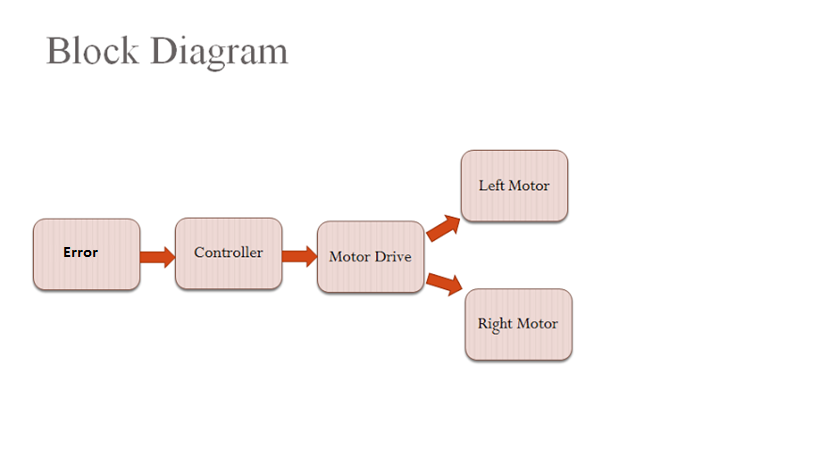
\includegraphics[scale = 1]{graphics/pid.png}
	\end{center}	
	
	\end{itemize}
	
	\pagebreak
	
	
	\begin{center}
		\textbf{\huge Theme Description} \\
	\end{center}
	
	Two firebird V are used where one of them is Master which is controlled manually and other one is slave which takes commands from computer as the video is processed using the webcam fitted at top of arena. Slave Bot will follow the Master Bot as the master bot moves, by avoiding the obstacles of green color that are moving in arena. Master Bot has markers of pink color and slave has of sky blue color, small rectangle in front and big one in rear.\\ \\
	
	\textbf{\large Web Cam}:
	
	To cover arena a web cam is fitted on roof of height of at least 8 feet. Web cam used is shown in figure
	
	\begin{center}	
	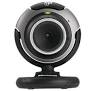
\includegraphics[scale = 1]{graphics/cam.jpg}\\
	\end{center}
	
	\textbf{\large Master Bot}: 
	
	Master bot have marker of pink color on it as shown in figure.\\
	
	\begin{center}  
	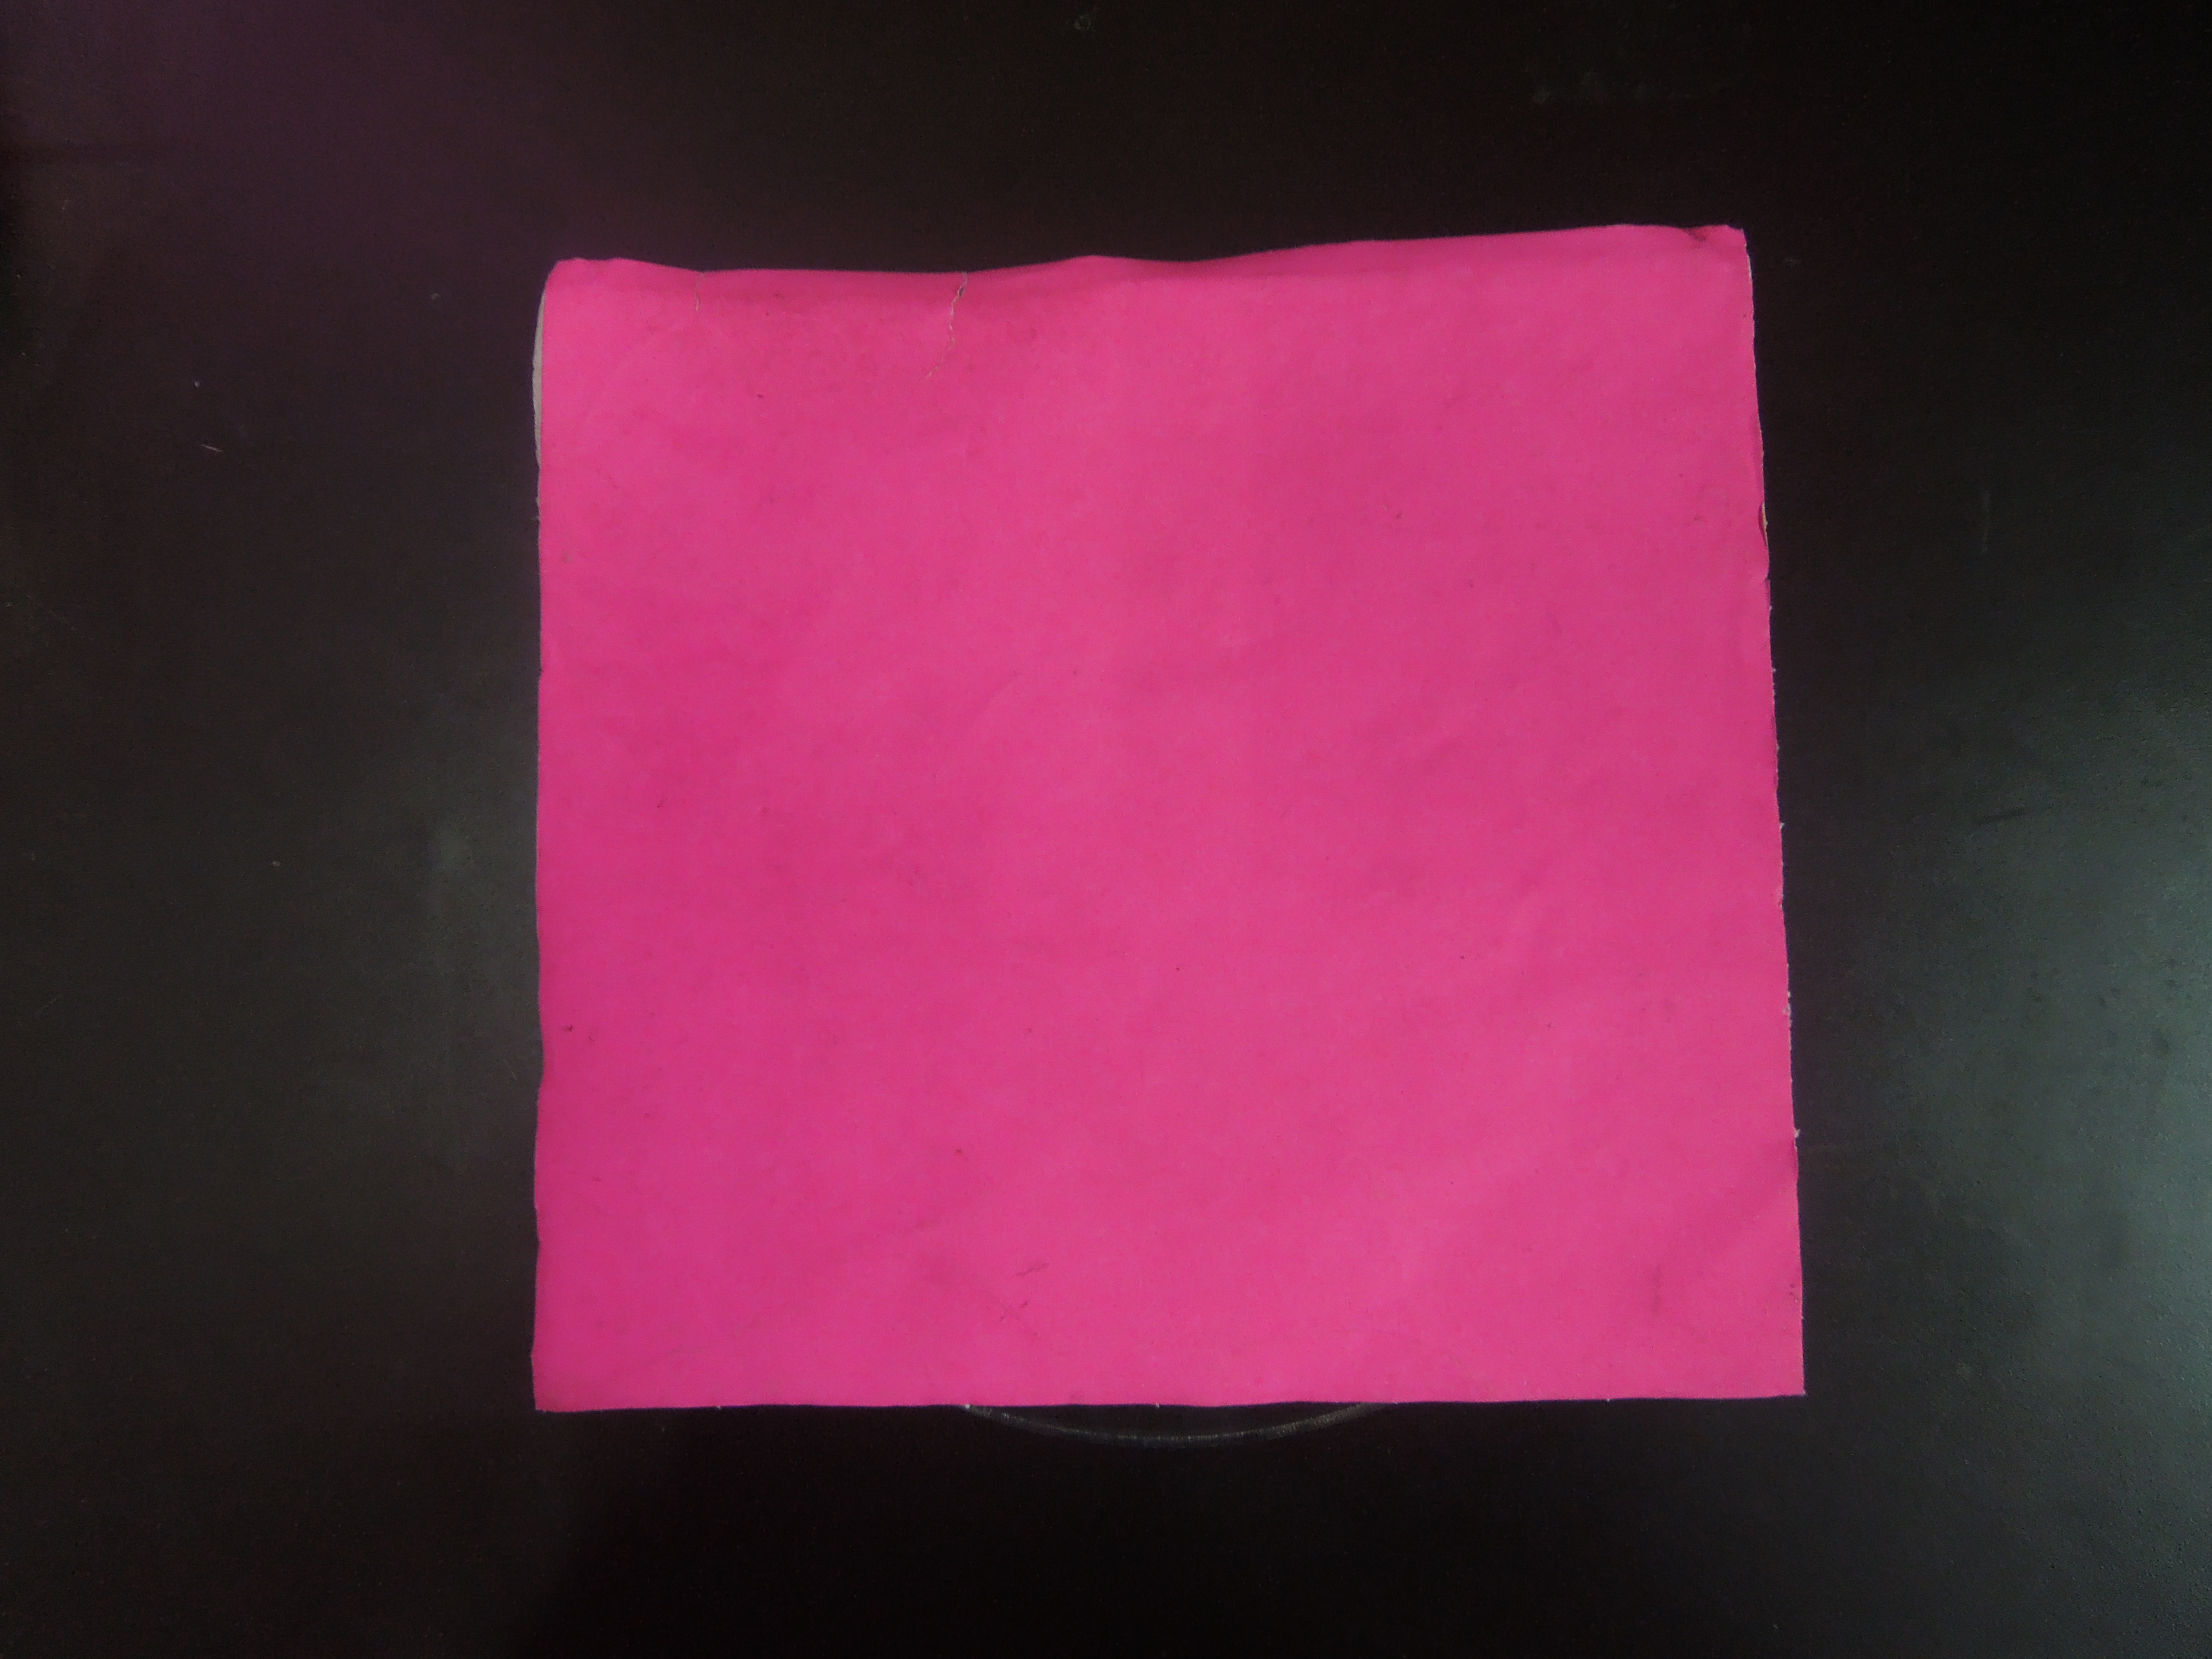
\includegraphics[scale = 0.05]{graphics/pics/DSCN0034.jpg}
	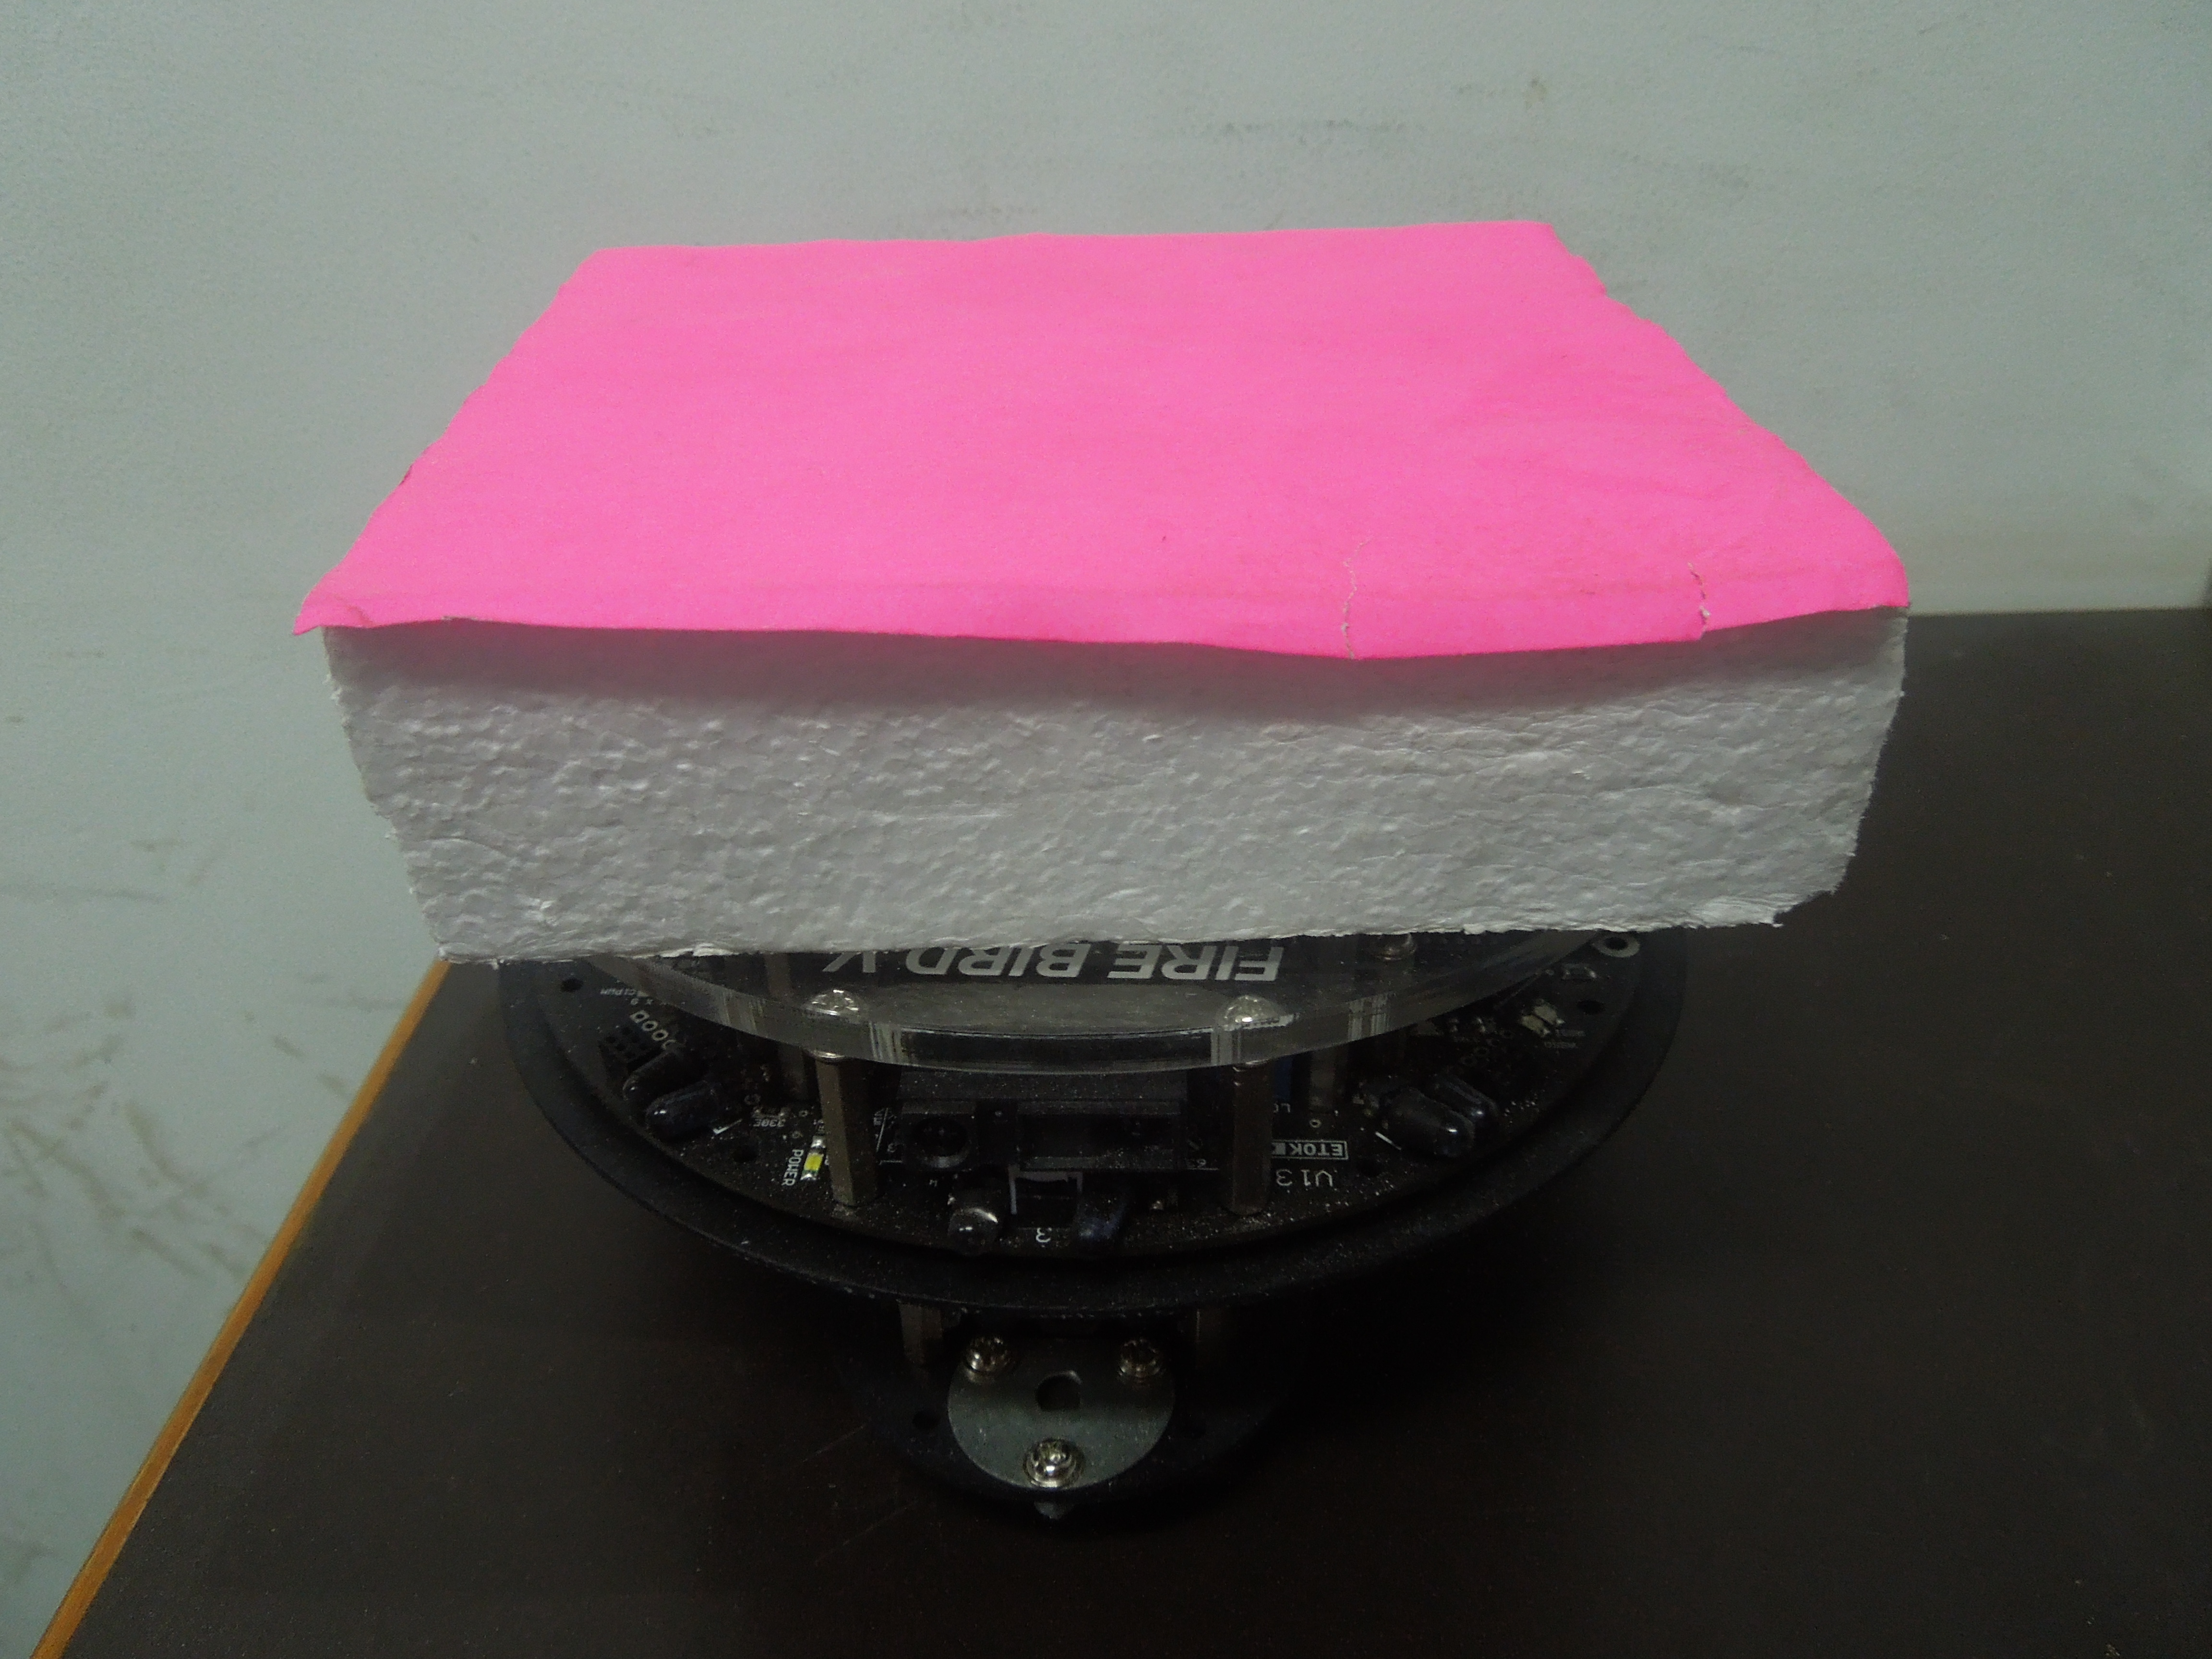
\includegraphics[scale = 0.05]{graphics/pics/DSCN0038.jpg} \\
	\end{center}
	
	\pagebreak	
    
    
    \textbf{\large Slave Bot}:	
	
	Slave Bot has two markers small rectangle in front and bigger rectangle in rear. To find the orientation of slave bot we use small one as a reference. Slave bot is shown in figure.\\	
	
	\begin{center}
	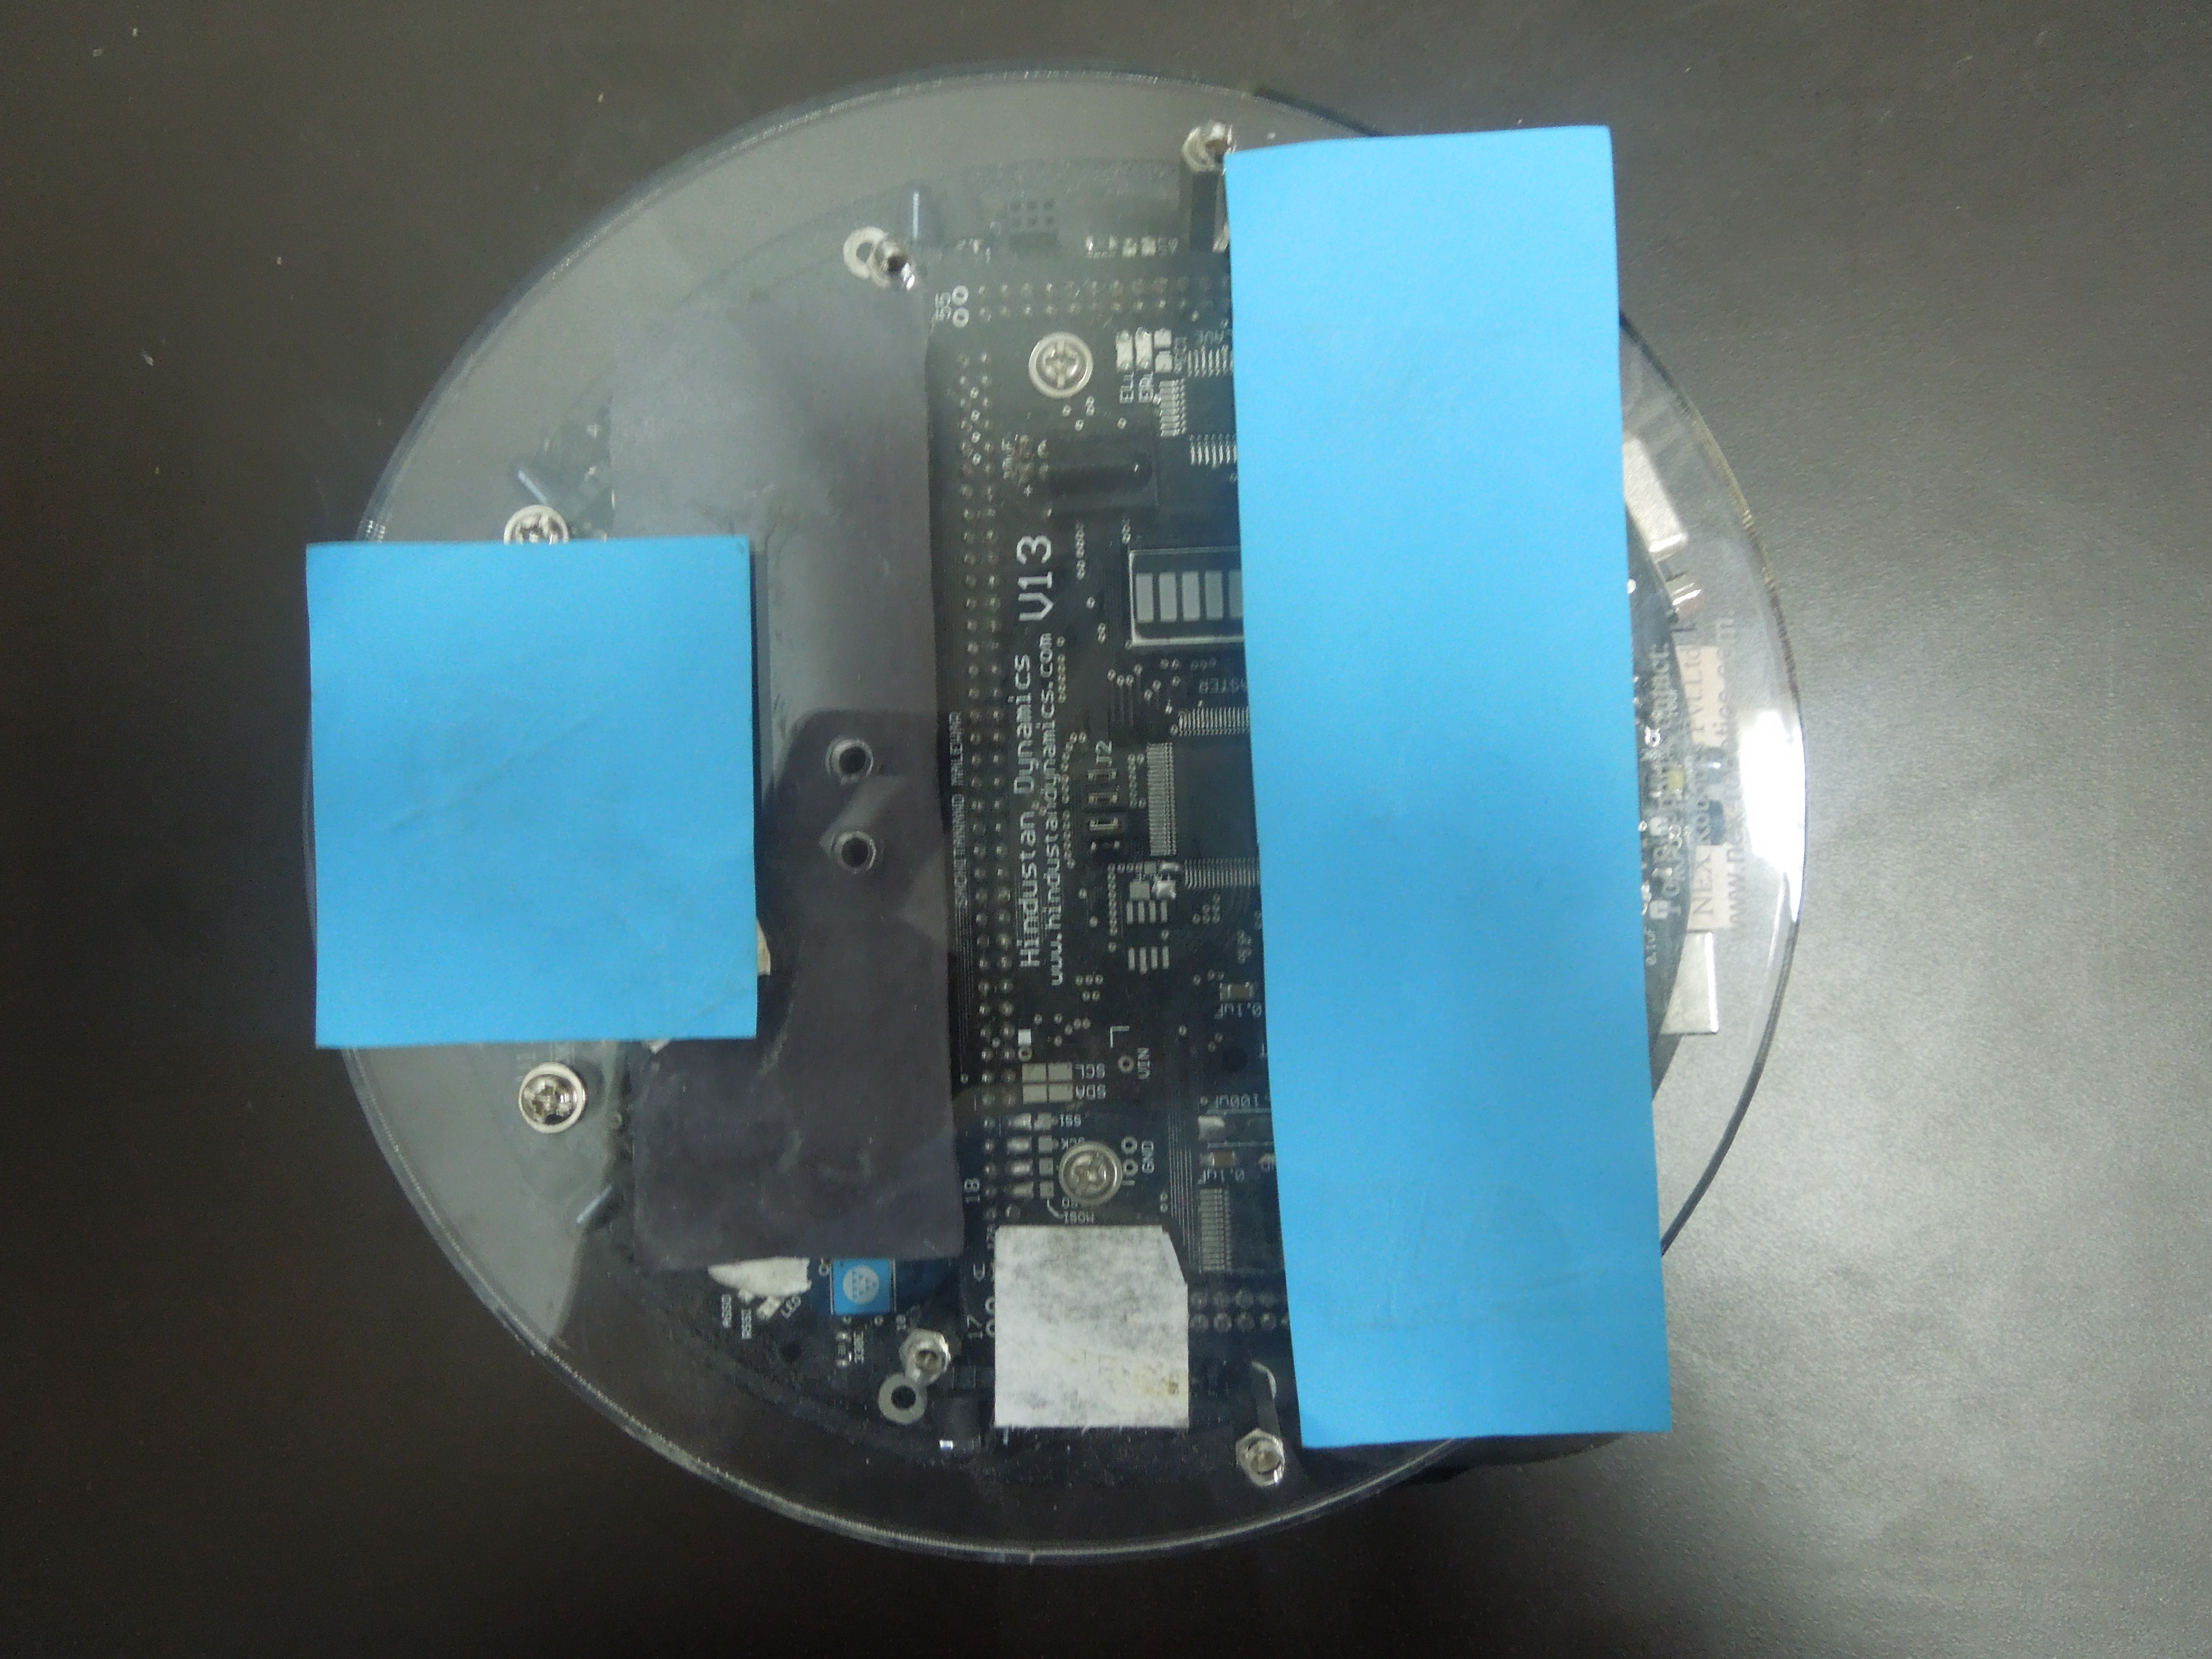
\includegraphics[scale = 0.05]{graphics/pics/DSCN0039.jpg}
	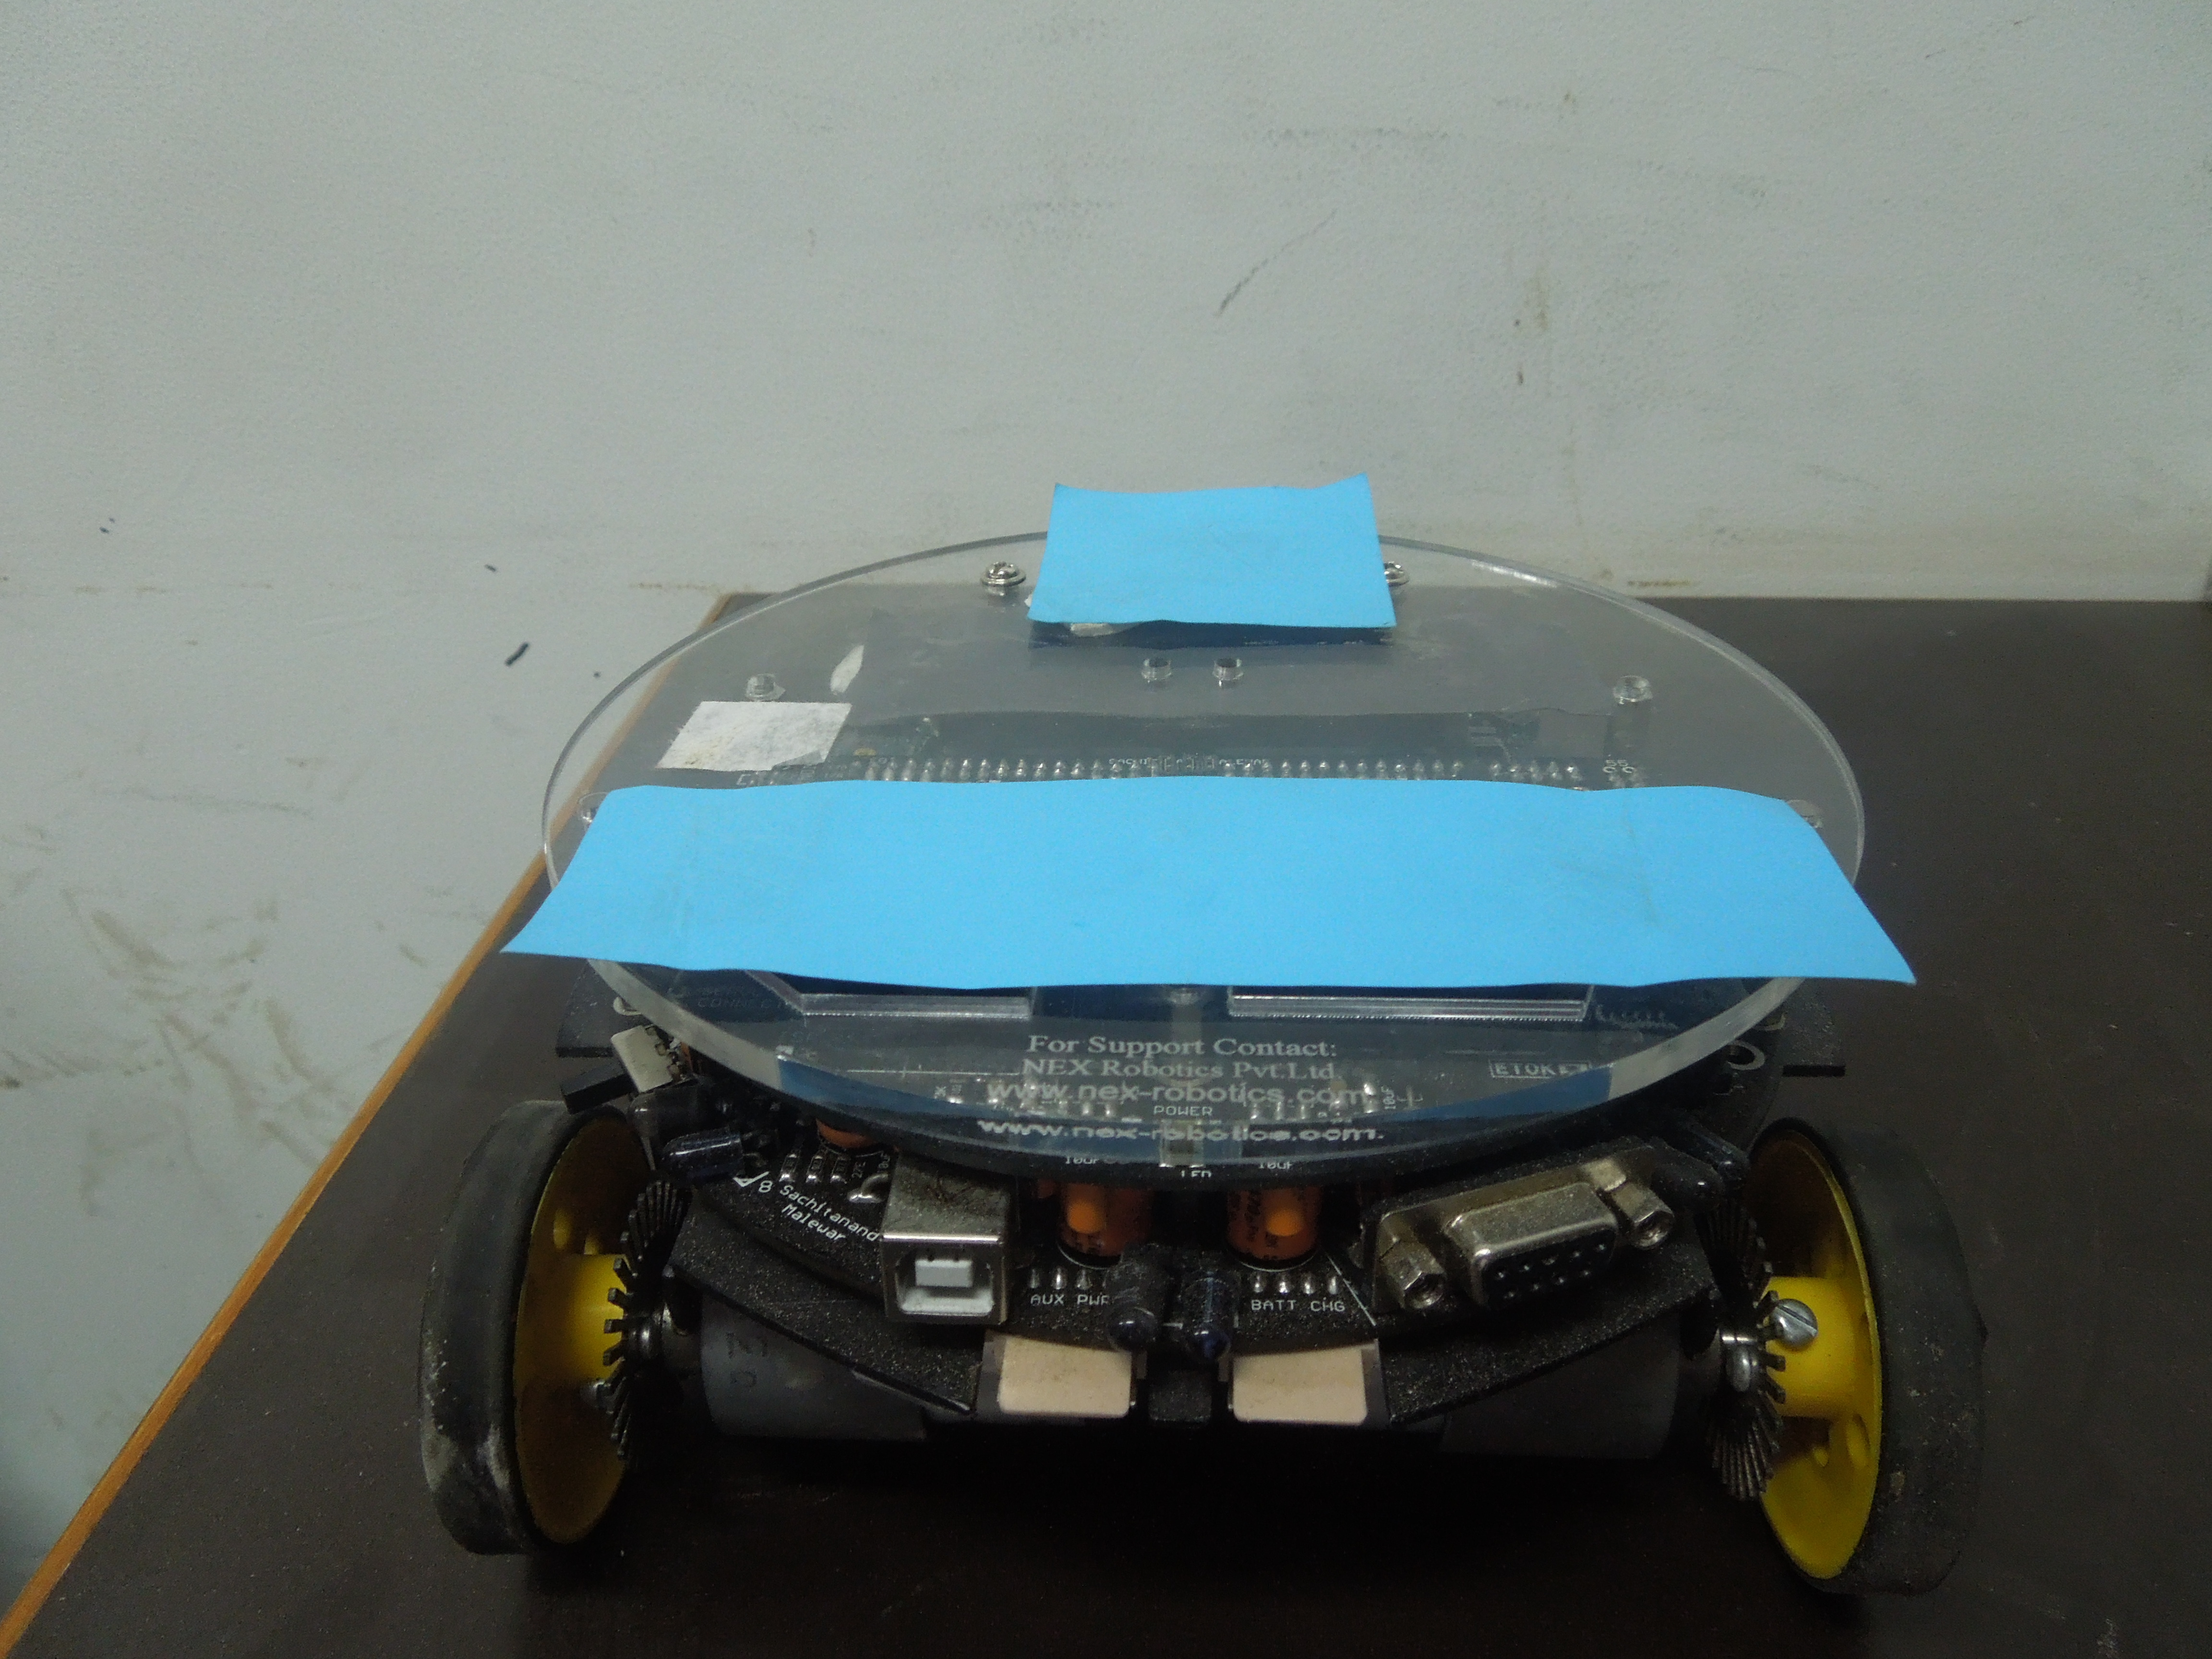
\includegraphics[scale = 0.05]{graphics/pics/DSCN0040.jpg} \\
	\end{center}
	
	\pagebreak
	
	
	\textbf{Walls}:
	
	To simulate real environments thermocol of green color is used as walls.\\
	
	\begin{center}
	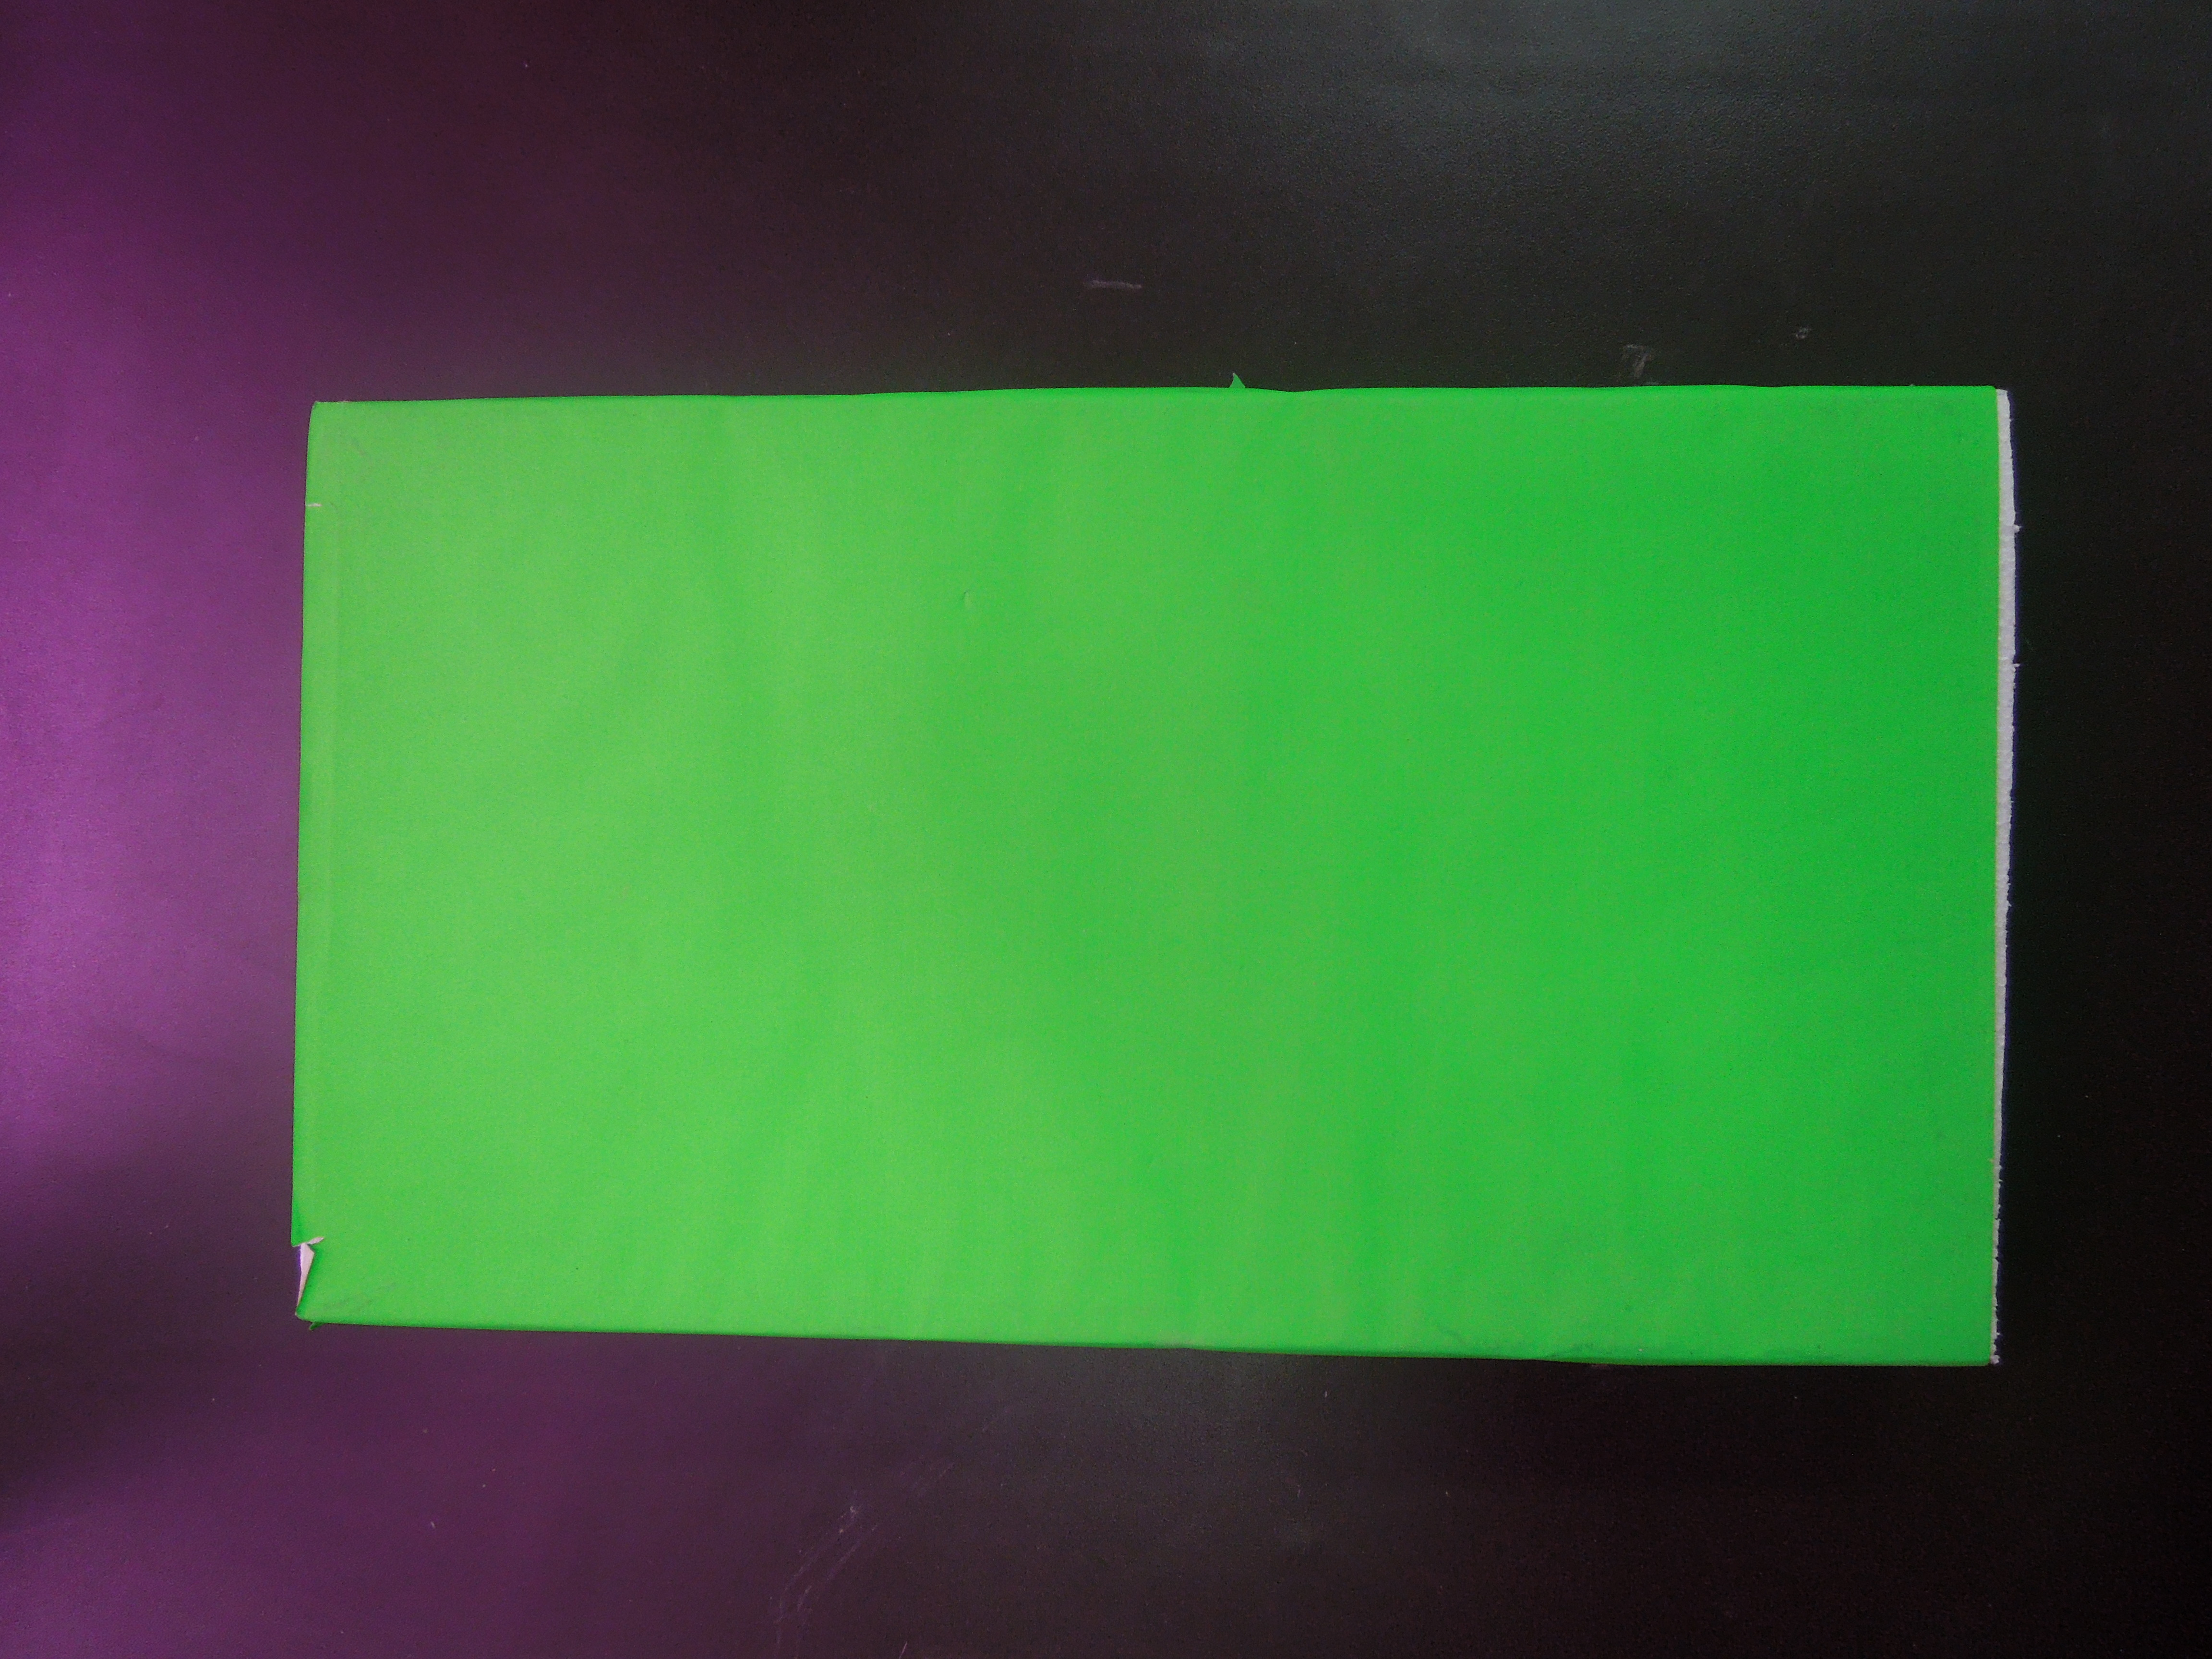
\includegraphics[scale = 0.05]{graphics/pics/DSCN0045.jpg}
	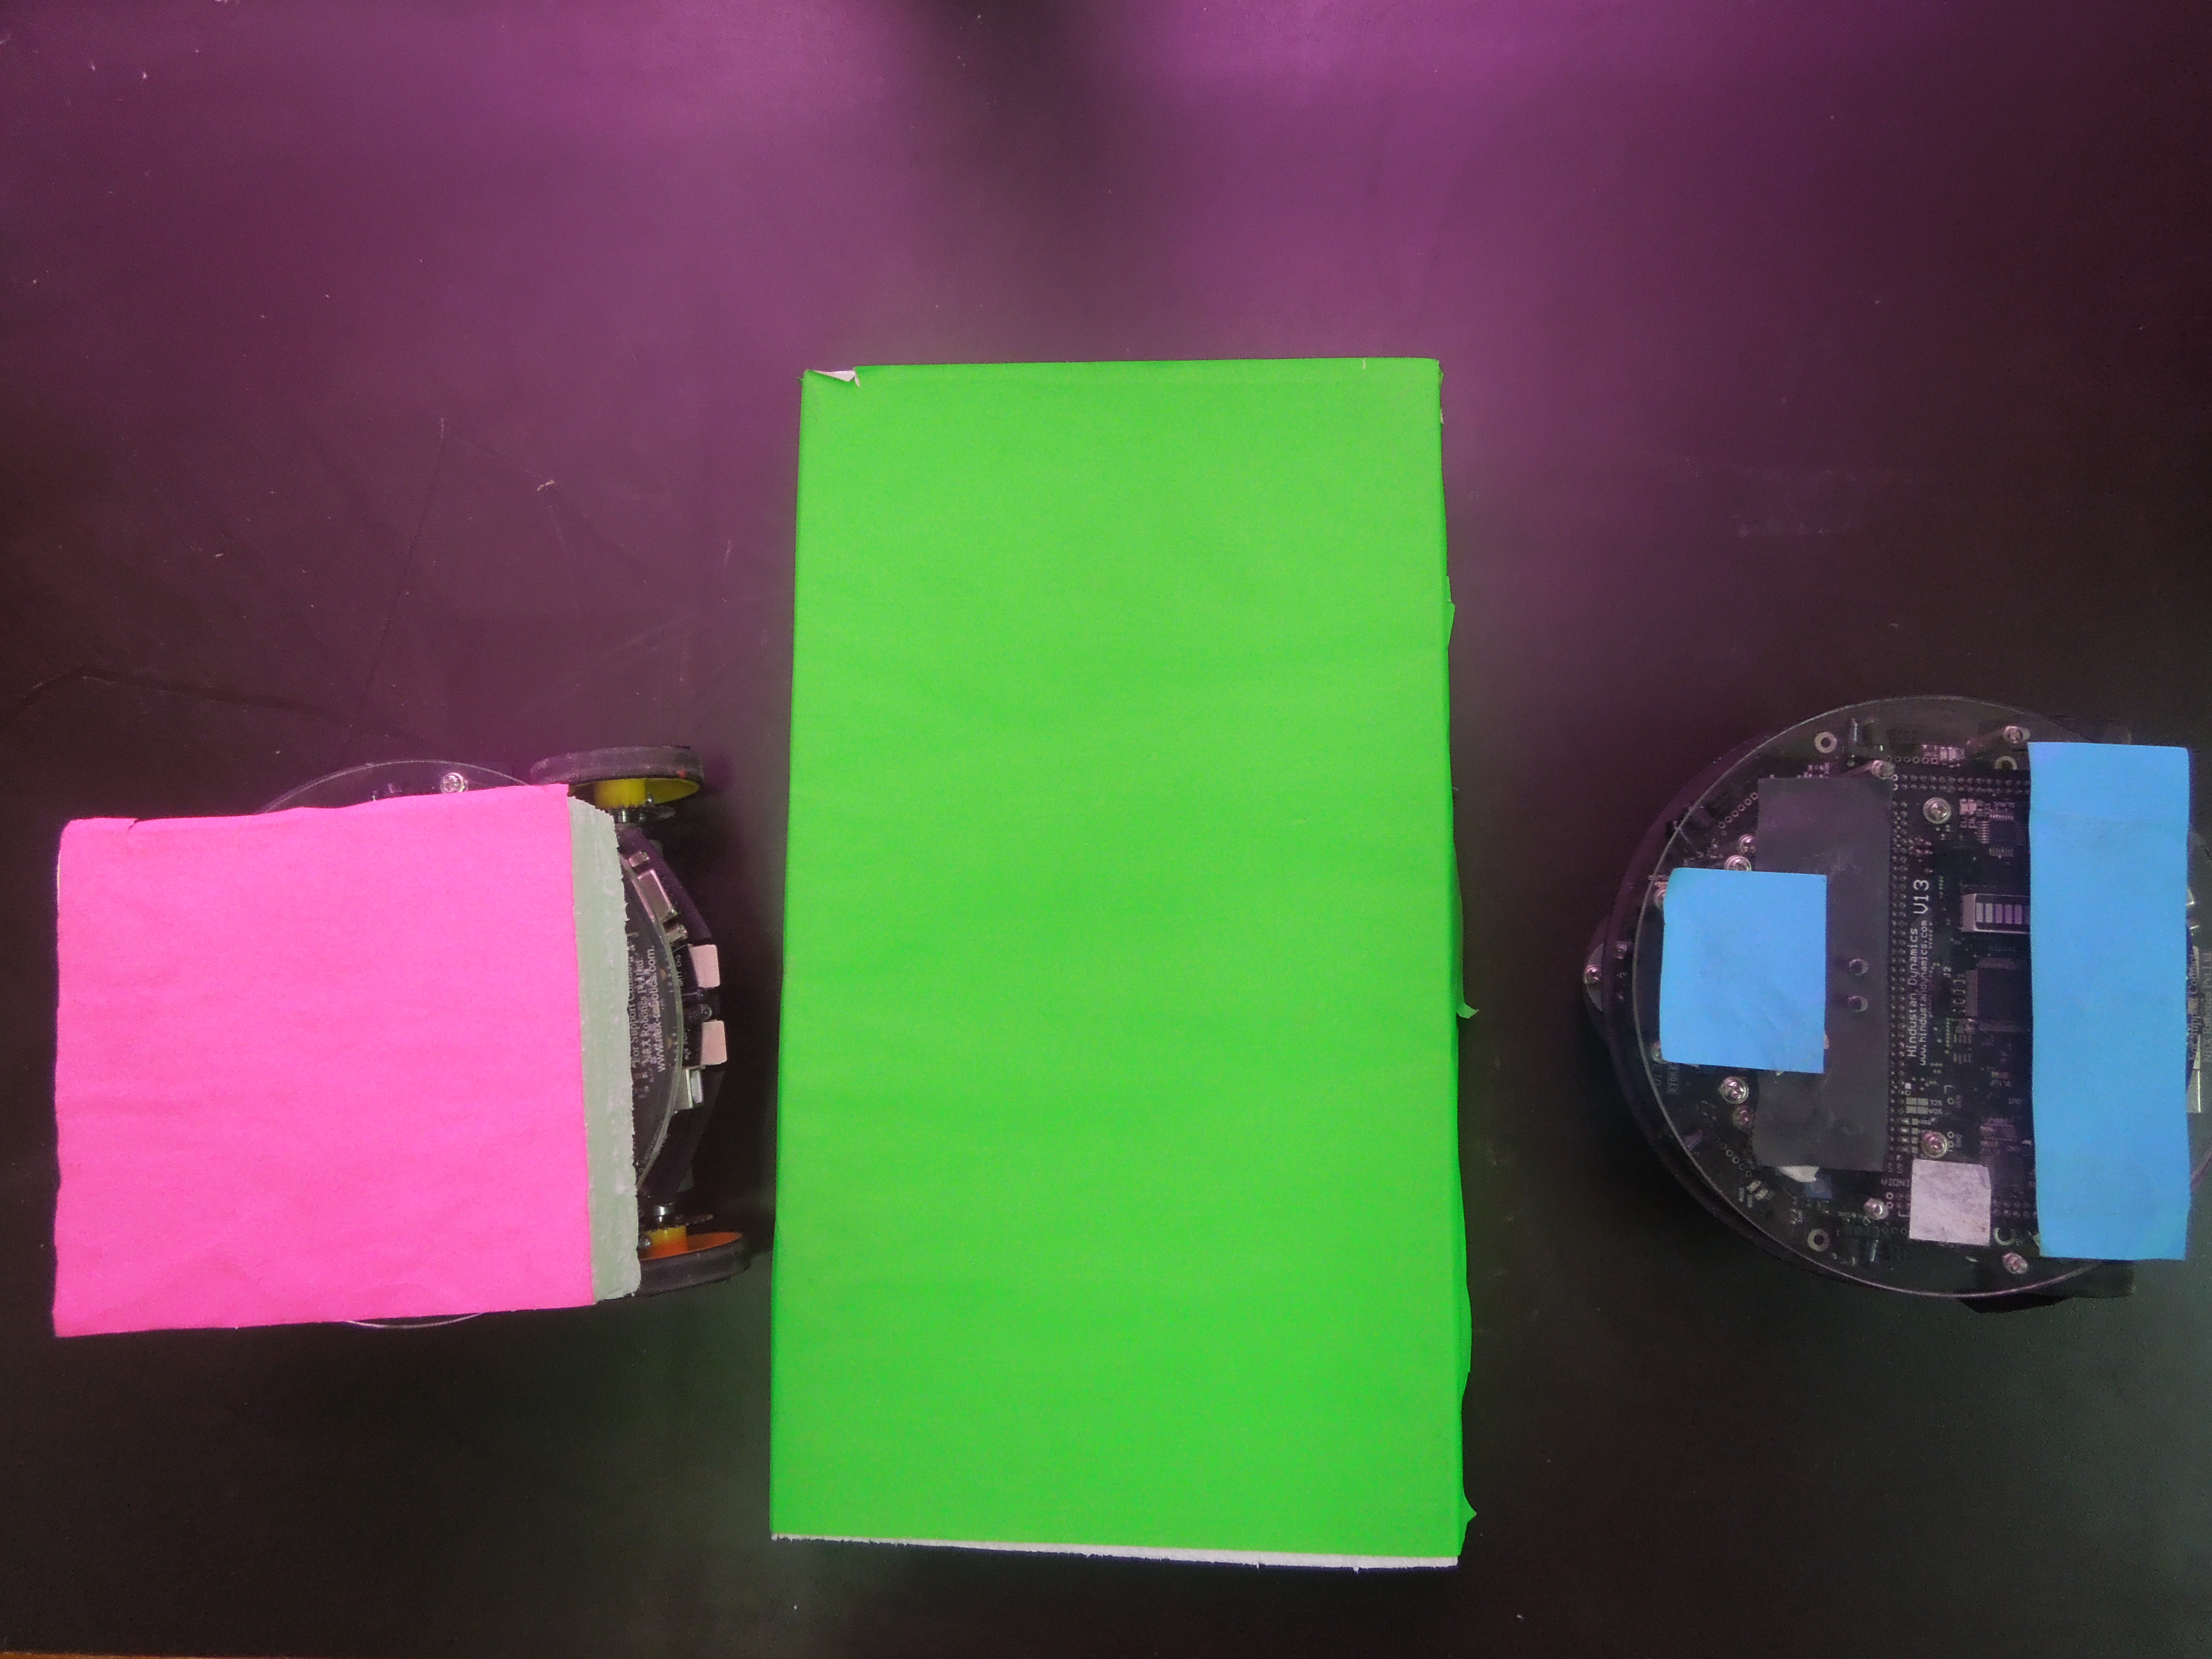
\includegraphics[scale = 0.05]{graphics/pics/DSCN0046.jpg}\\
	\end{center}
	
	\pagebreak
	
	
	\textbf{\large Setup of Arena to simulate real environment is as shown in figure.}
	
	\begin{center}
	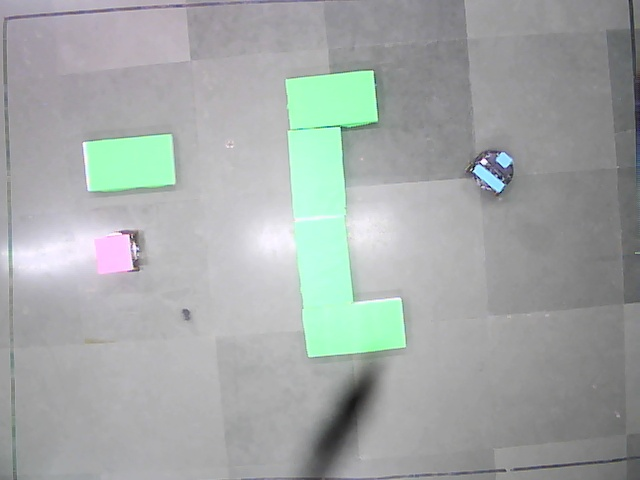
\includegraphics[scale = 0.8]{graphics/case1/cap_image.jpeg}\\
	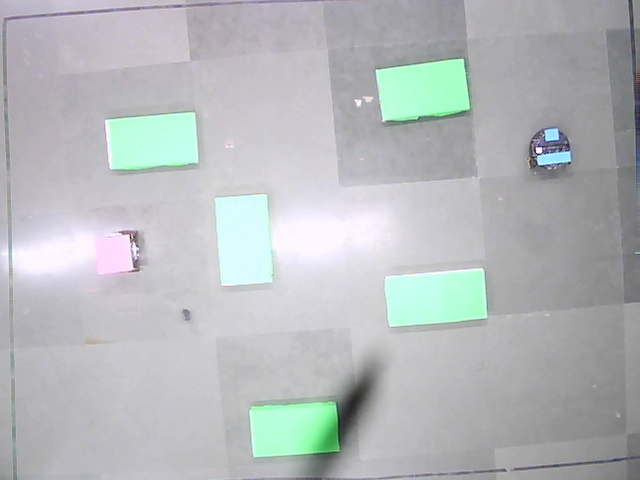
\includegraphics[scale = 0.8]{graphics/case2/cap_image.jpeg}\\
	\end{center}
	
	\pagebreak
	
	
	\begin{center}
		\textbf{\huge Algorithm} \\
	\end{center}
	
	\begin{itemize}
	\item First we fixed a web cam on the roof at least 8 feet height and created a boundary which is covered by webcam. Now webcam is initialized to capture the video of the floor,for this OpenCV video capture function is used. Then we read frames from video at every interval of 1/80 sec so that we can get 10-12 frames per second for image processing. 
	\item The video captured is in RGB format,so for greater processing RGB image is converted into HSV format.
	\item Then hsv image is send to the bot position and destination function where Master and slave Bot markers are masked and centroid of contours of those markers is stored for further use. 
	\item Now for detection of walls on floor hsv image is send to the wall detection function where walls are masked and contours of walls is found. 
	\item To be compatible with grid map based path morphological operation of closing following with dilation is done on walls. So the size of walls increased to its true size. 
	\item Now to create a grid map across those walls this dilated image is send to grid map of walls function. 
	\item For this dilated image is divided into grids of 30*30. And center of every grid is checked if it is white then 1 is placed at respective place of grid matrix of 30*30 else its 0 and boundaries of matrix is default 1 to be in safer side. 
	\item Now a bot route function is called which returns the path to the destination point having walls in it. 
	\item To find shortest path to the destination heapq algorithm is used. 
	\item In heapq all the path to the destination are stored in heap and shortest path is returned on the basis of shortest length. 
	\item As in video processing path is created at every instant so we update new path only if present path length is less than the last path. 
	\item To show the path following we call route draw function which draws path from the slave bot to destination on frames which can be seen as a reference on screen. 
	\item After it bot traverse function is called which handles the slave bot movements, where orientation function is called. 
	\item As the returned path is links of coordinates of grids. So for movements of path angle between the lines of slave bots rear marker to route path’s first coordinate and between slave bot front and rear markers is taken using the mathematical function with the help of slope of both line. 
	\item As this angle is fed to PID controller as error input which process this value and return correction. 
	\item If correction is negative then bot moves rights if its positive then left. 
	\item To send these values to the slave bot serial communication via xbee is used. 
	\item If pid correction approaches zero then slave bots moves forward. 
	\item So if slave bot reaches to cell then coordinates of next cell from path is updated to follow so in that way local destination point is followed to reach global destination. 
	\item If bot reaches near to final destination then stop.
	\end{itemize}
	
	\pagebreak
	
	
	\textbf{Steps involved in Image Processing}
	
	\begin{itemize}
		\item	Capturing Video of the Arena from external web cam situated on top of Arena.
		\item	Markers placed on Master and slave firebird V
		\item	Sky blue color small rectangle size shows the front of slave and Bigger one for rear end of slave firebird
		\item	Pink Marker for Master Firebird V.
		\item	Walls are defined by green color.
		\item	Centroid of contours of masked Master, slave and walls are stored.
		\item	Frames from video is converted in to grid map.
		\item	Walls are mapped to the grid matrix by denoting 1 if there is wall else 0. Boundaries are 1 in default.
		\item	Shortest path is find using heapq algorithm for maze solving on grid.
		\item	Angle between Slave markers and path is fed to the PID controller to get correct speed of Motors.
		\item	PID controlled commands are given to the motor to follow the path.
		\item	Check the slave rear markers if it has reached near the destination then stop.
	\end{itemize}
	
	\pagebreak	
	
	
	\begin{center}
		\textbf{\huge Implementation} \\
	\end{center}
	
	\textbf{HSV Format}:
	
	After capturing frame from video it is converted into HSV. Which is shown in figure
	
	\begin{center}
	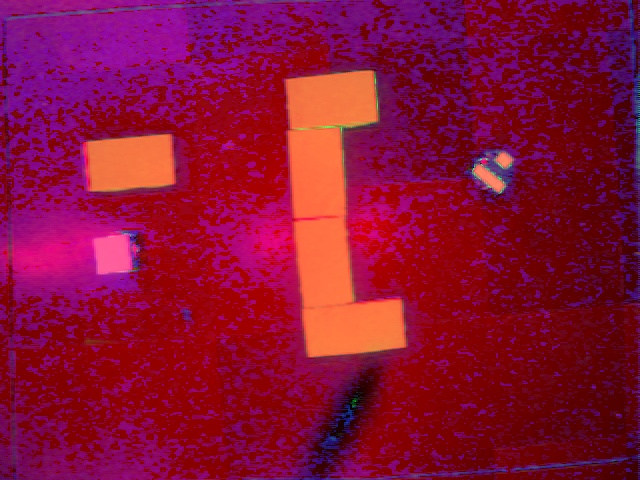
\includegraphics[scale = 0.8]{graphics/case1/have_video.jpeg}\\
	\end{center}
	
	\pagebreak
	
	
	\textbf{Destination masking}:	
	
	To locate destination point or Master Bot, masking of pink color is done on hsv image of frames captured by video as shown in figure.
	
	\begin{center}
	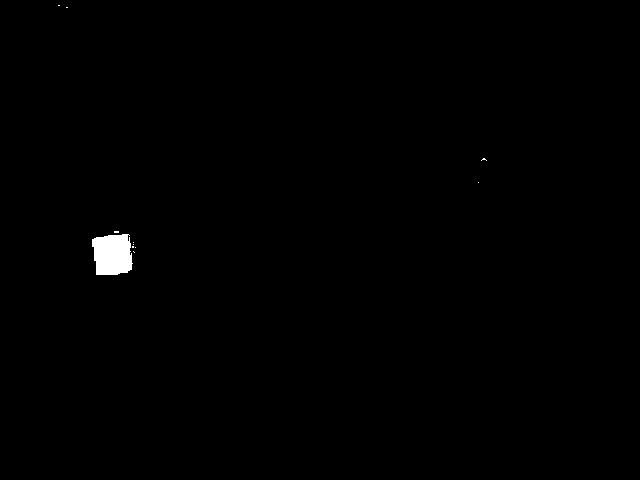
\includegraphics[scale = 0.8]{graphics/case1/destination_mask.jpeg}\\
	\end{center}
	
	\pagebreak
	
	
	\textbf{Source masking}:
	
	To locate source or slave bot markers are masked. Slave bot markers are of sky blue color. Masked area is shown in figure.
	
	\begin{center}
	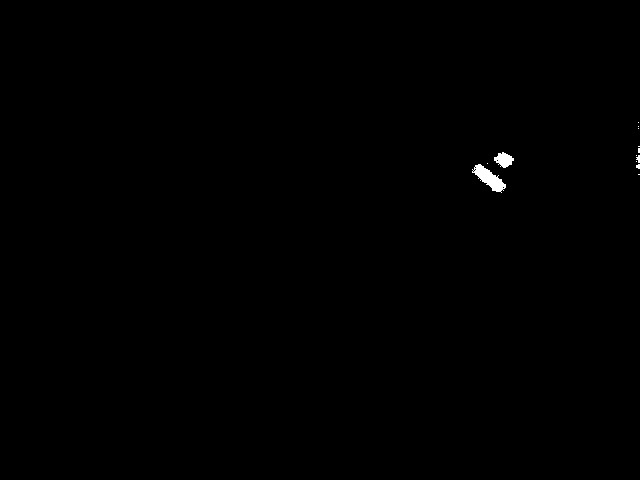
\includegraphics[scale =1]{graphics/case1/slave_mask.jpeg}\\
	\end{center}
	
	\pagebreak
	
	
	\textbf{Wall Detection}:
	
	To detect walls masking of green color is done. Mask area of walls is given by figure. And then morphological operation is done closing followed by dilation to use for avoiding obstacle.
	
	\begin{center}
	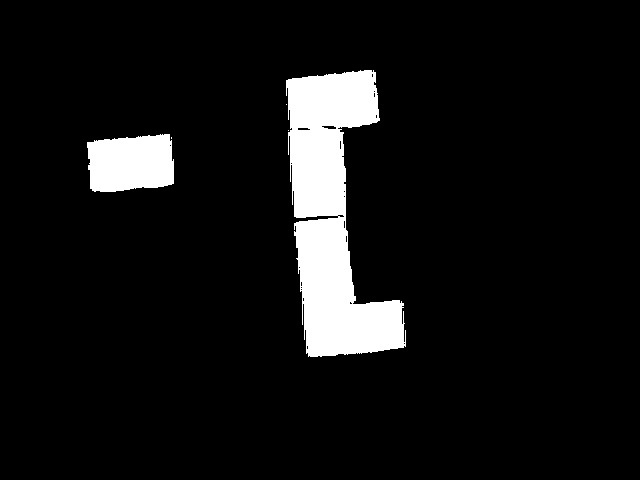
\includegraphics[scale = 0.8]{graphics/case1/walls_mask.jpeg}\\
	\end{center}
	
	\pagebreak	
	
	
	\textbf{Grid Draw}:
	
	For path mapping image is converted into grid of 30*30. As you can see in figure 
	
	\begin{center}
	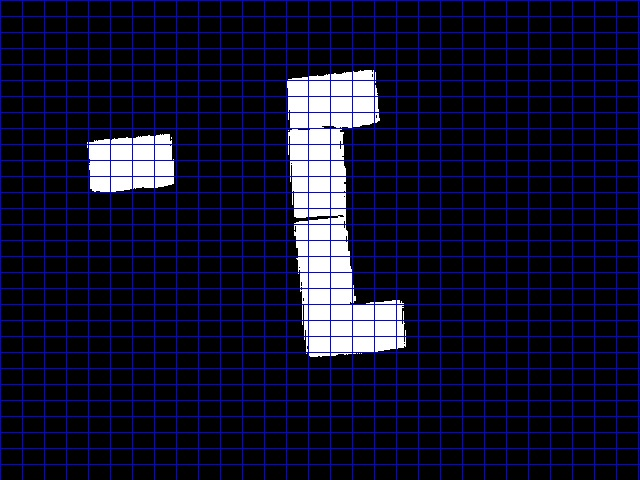
\includegraphics[scale = 0.8]{graphics/case1/walls_mask11.jpg}\\
	\end{center}
	
	\pagebreak
	
	
	\textbf{Grid map}:
	
	A grid map is also initialized to find the path from source to destination having obstacles on it. Grid map is a 30*30 matrix in which if center of grids from dilated image of walls is white then 1 is placed at respective place in matrix else it is 0. Boundaries are 1 as default just to be in safer side for path finding. Grid matrix across walls is shown here:\\
	
	\begin{center}
	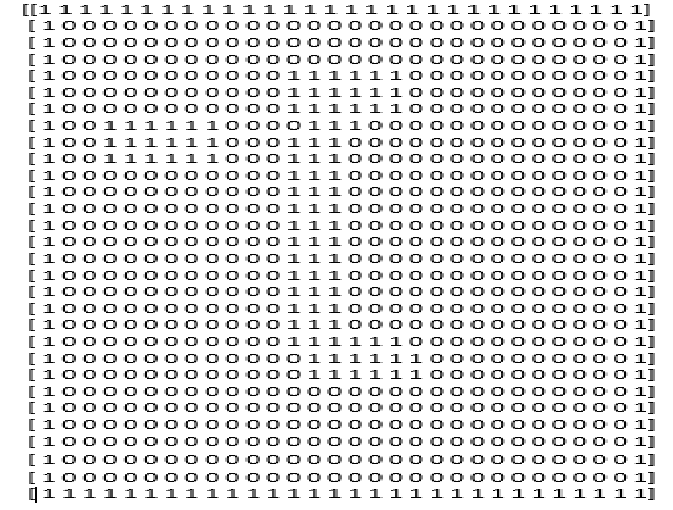
\includegraphics[scale = 0.8]{graphics/grid_map.png}\\
	\end{center}
	
	\pagebreak	
	
	
	\textbf{Mapping Path}:
	
	Path is mapped using the grid map created. To find the shortest path heapq algorithm is used. In heapq all path from source to destination is stored into the min heap and shortest path is returned on the basis of shortest length of path. A path mapped from source to destination avoiding obstacles are shown in figure\\
	
	\begin{center}
	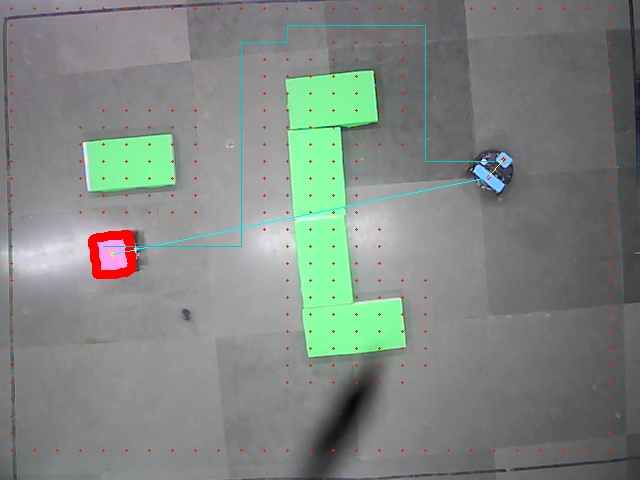
\includegraphics[scale = 0.8]{graphics/case1/path_route.jpeg}\\
	\end{center}
		
	Red points denotes unreachable grid. A light blue line from start to end location to show where to reach. And light green color line following grids with avoiding obstacles is the path will slave bot will follow.
	
	\pagebreak
	
	
	\textbf{Motion of Bot}:
	
	For movement of Bot angle theta shown in figure is fed to the PID 
	controller.\\
	
	\begin{center}
	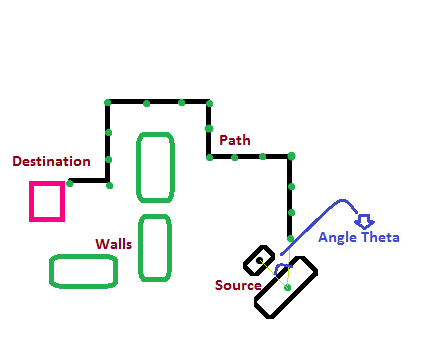
\includegraphics[scale = 1.3]{graphics/pid_error.png}\\
	\end{center}
		
	angle is negative if it is on left side of the path and positive if on right side of path. This results in a negative and positive error. So PID controller use these value and return a correction value which added to motor speed which helps to control the fire bird to be in path.
	To send these values to the firebird xbee communication is used.
	
	\pagebreak
	
	
	\begin{center}
		\textbf{\huge Flow Chart} \\
	\end{center}
	
	\textbf{\Large Overview of Algorithm}:\\
	
	\begin{center}
	\includegraphics[scale = 1.4]{graphics/drawing1.jpg}\\
	\end{center}
	
	\textbf{\Large Working Of PID Controller}:\\
	
	\begin{center}
	\includegraphics[scale = 1.3]{graphics/drawing2.jpg}\\
	\end{center}
	
	\pagebreak
	
	
	\textbf{\Large Finding Shortest Path}:\\ \\
	
	\begin{center}
	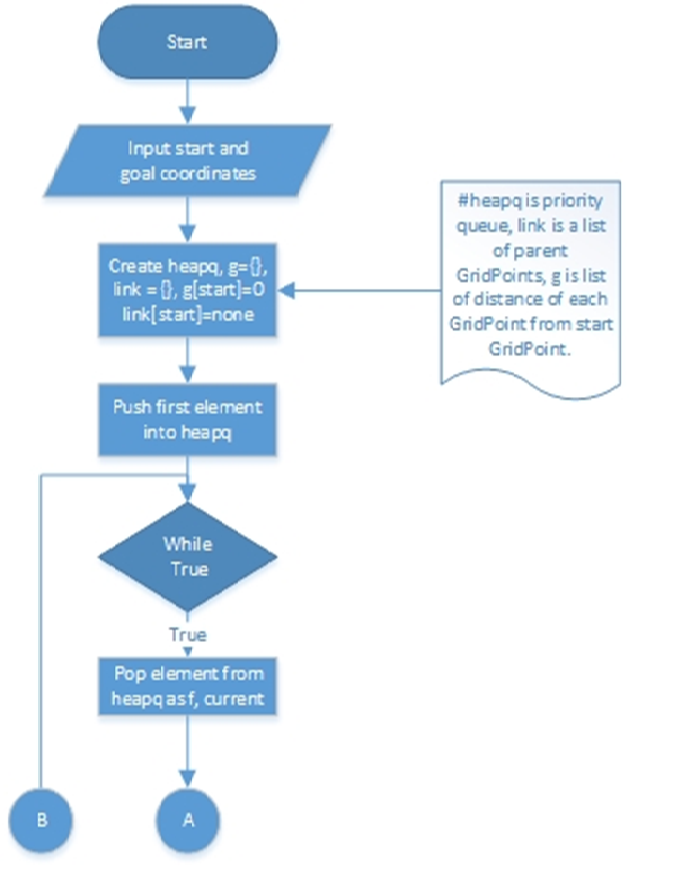
\includegraphics[scale = 0.8]{graphics/movement_flow.png}\\
    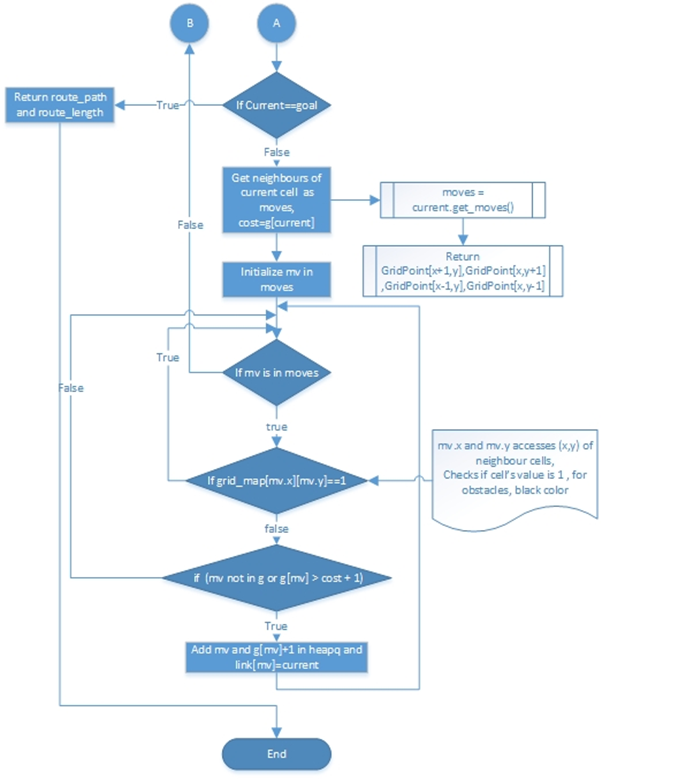
\includegraphics[scale = 1.1]{graphics/movement_flow2.jpg}\\
	\end{center}
	
	\pagebreak
	
	
	\begin{center}
		\textbf{\huge Results and Discussion} \\
	\end{center}
	
	\begin{itemize}
	\item Using image processing we are able to control the slave bot to follow master bot with avoiding obstacles.
	\item For Masking different color we used hsv format of color. 
	\item We used grid map based path planning which gives problem in returning path which are near to walls. 
	\item To overcome with those problem we tried to dilate the walls. But it is not a good practice. 
	\item We can by pass this by planning a path on the basis of local path then global path based planning. 
	\item PID controller for controlling bot using image processing is working fine. 
	\end{itemize}

	\pagebreak


	\begin{center}
		\textbf{\huge Problems Faced} \\
	\end{center}

	During the project we faced following problem.

	\begin{itemize}

		\item Masking of color is toughest challenge. To handle it we created a hsv track-bar tool where we can vary the HSV range individually to mask a color.
		\item Choosing color combination for markers as lighting condition giving problem.
		\item To find the orientation of path respective to path at every  instant.
		\item Mapping a path at every instant results in different source grid point. As there are more than one shortest path to the destination on the basis of grid map. 
		
	\end{itemize}
	
	\pagebreak
	
	
	\begin{center}
		\textbf{\huge References} \\
	\end{center}
	
	\begin{itemize}
	
		\item http://www.coursera.org/course/conrob
		\item http://www.robotics.in/tutorials/categ/avr/pid
		\item https://www.docs.python.org
		\item https://www.docs.opencv.org
		\item https://stackoverflow.com/
	
	\end{itemize}
	
\end{document}
